\section[递归最小二乘(与卡尔曼滤波)]{递归最小二乘(与卡尔曼滤波)\\Recursive Least Squares(and Kalman Filter)}
例4.4 \quad 假设我们已经计算了99个数$b_1,...,b_{99}$的平均数$\hat{x}_{99}$,出现一个新的数$b_{100}$,我们如何在不把前99个数再重新加一遍的情况下得到一个新的平均值$\hat{x}_{100}$(加上$b_{100}$)?我们只想利用$\hat{x}_{99}$和$b_100$。

这是新旧正确的组合$\hat{x}_{100}$,表现为两种形式:

新平均值 
\begin{equation}
\hat{x}_{100}=\frac{99}{100}\hat{x}_{99}+\frac{1}{100}b_{100}=\hat{x}_{99}+\frac{1}{100}(b_{100}-\hat{x}_{99})
\end{equation}
公式中第一项$\frac{99}{100}\hat{x}_{99}$是$(\frac{99}{100})$乘以$(\frac{1}{99})$再乘以$(b_1+b_2+...+b_{99})$,约去99,就是$(\frac{1}{100})$乘以这99个数的和(没有重新加一次!),加上额外的$(\frac{1}{100})$给出所有b的和,再除以100,这就是正确的平均值。

我们更喜欢第二张形式的递推公式(4.24)。通过复杂的创新$b_{100}-\hat{x}_{99}$得到右边更新的$\hat{x}_{99}$,这个创新表明了有多少“新信息”在$b_{100}$中。当$b_{100}$等于旧平均数,创新为0,在这种情况下,更新的$\hat{x}_{100}$就是原来的$\hat{x}_{99}$,校正=预测。

创新是将这个更新公式(4.24)乘以$\frac{1}{100}$,这个增益系数使这个公式正确。想到同样的方法$Ax=b$,从最小二乘解决方程$A_{old}x=b_{old}$入手,新的信息加入,新的观测值$b_{new}$,组合方程$Ax=b$通过最小二乘解出,组合系统为:
\begin{equation}
\begin{bmatrix}
A_{old} \\ A_{new}
\end{bmatrix}
\begin{bmatrix}
x
\end{bmatrix}
\begin{bmatrix}
b_{old} \\ b_{new}
\end{bmatrix}
\end{equation}
引导$\hat{x}_{new}$。

估值$\hat{x}_{new}$从整个系统$Ax=b$得到,在$b_{old}$中的数据仍然有助于$\hat{x}_{new}$,但是我们不想做相同的计算两次。

问题4.1  \quad 我们能否仅用$A_{new}$和$b_{new}$更新$\hat{x}_{old}$和$\hat{x}_{new}$?采取$C=I$
答案 \quad  既然$A^T=\begin{bmatrix} A^T_{old} & A^T_{new}\end{bmatrix}$,我们需要$A^TA$在正常方程:
\begin{equation}
A^TA=A^T_{old}A_{old}+A^T_{new}A_{new}=(known)+(new)
\end{equation}
然后在右边我们需要$A^Tb$,也涉及到新旧值:
\begin{equation}
A^Tb=A^T_{old}b_{old}+A^T_{new}b_{new}=A^T_{old}A_{old}\hat{x}_{old}+A^T_{new}b_{new}
\end{equation}

用$A^TA-A^T_{new}A_{new}$代替$A^T_{old}A_{old}$,然后乘以$(A^TA)^{-1}$找到$\hat{x}_{new}$:
\begin{equation*}
\hat{x}_{new}=(A^TA)^{-1}((A^TA-A^T_{new}A_{new})\hat{x}_{old}+A^T_{new}b_{new})
\end{equation*}

这个更新的公式简化了从原来的值产生新的$\hat{x}$,递推:
\begin{equation}
\hat{x}_{new}=\hat{x}_{old}+(A^TA)^{-1}A^T_{new}(b_{new}-A_{new}\hat{x}_{old})
\end{equation}
最后一项$b_{new}-A_{new}\hat{x}_{old}$是更新,这是我们对于观测值$b_{new}$的预测误差。如果误差为零,数据$b_{new}$与旧估计是完全一致的,没有理由去改变,因此$\hat{x}_{new}=\hat{x}_{old}$。

通常更新项$b_{new}-A_{new}\hat{x}_{old}$不为零,然后(4.28)乘上增益矩阵$K=(A^TA)^{-1}A^T_{new}$找到$\hat{x}$中的变化,增益矩阵是“放大器”,由K(卡尔曼)提出。注意到$A^TA$和$\hat{x}$在更新(4.26)和(4.28)有大小n,比m小。

例4.5 \quad (例4.4完整版)平均值$\hat{u}_{99}=\frac{1}{99}(b_1+...+b_99)$是一元99个方程的最小二乘解,99由1矩阵$A_{old}$是所有的:
\begin{equation*}
\begin{bmatrix}
1 \\ \dots \\ 1
\end{bmatrix}
u=
\begin{bmatrix}
b_1 \\ \dots \\ b_{99}
\end{bmatrix}
A^T_{old}A_{old}\hat{x}_{old}=A^T_{old}b_{old}
\end{equation*}
为:
\begin{equation*}
99\hat{x}_{old}=b_1+...+b_{99}
\end{equation*}
第100个方程是$u=b_{100}=b_{new}$,新的一行是$A_{new}=[1]$,检查所有:

(4.26)更新$A^TA$:
\begin{equation*}
A^TA=99(old)+1(new)=100
\end{equation*}

(4.28)更新$\hat{x}$:
\begin{equation*}
\hat{x}_{100}=\hat{x}_{99}+\frac{1}{100}(b_{new}-A_{new}\hat{x}_{old})=\hat{x}_{99}+\frac{1}{100}(\hat{x}_{100}-\hat{x}_{99})
\end{equation*}

更新的公式与方程(4.24)匹配,增益K是$(A^TA)^{-1}A_{new}=\frac{1}{100}$。

重要的是,你可能认为$A^TA=100$仅仅是对$\hat{x}_{100}$有用的一步,一点也不是,在最小二乘中,$A^TA$(及其逆)是比答案本身更有意义!当我们包含加权矩阵$C=\Sigma^{-1}$时,更新方程(4.26)给出$A^TCA$。我们已经知道为什么想要这个矩阵:逆矩阵$A^TCA=A^T\Sigma^{-1}A$量测$\hat{x}$的可信度P。

在这100个方程的例子中,$b_i$具有相等的可信度,它们有相同的方差$\sigma^2$,来自“标准”正态分布,它们都有$\sigma^2=1$,加权矩阵是$C=I$(正如我们所选),然后$A^TCA=100$的逆量测它们平均值$\hat{x}_{100}$的可信度,如果100个样本有相同的$\sigma^2$,它们的平均值有方差$\sigma^2/100$,当递推最小二乘更新$\hat{x}$时更新矩阵$P=(A^T\Sigma^{-1}A)^{-1}$。

	\subsection[卡尔曼滤波实例]{卡尔曼滤波实例\\Kalman Filter by Example}
	卡尔曼滤波应用在时变最小二乘中,状态x是不断变化的。在离散时间中,我们在每一个$t=i$时间下产生一个估计$\hat{x}_i$,早期的测量仍然给出关于目前状态的信息,因为这种状态是相关的,所以那些$b's$被包含在计算$\hat{x}_i$中。它们可能作用小一些,但是仍然起作用。
	
	例4.6 \quad  有一个未知数x,你的心率,医生第一次测量为$b_1$,之后测量为$b_2$,如果没有理由预测改变,最好的估计$\hat{x}$将是平均数$\frac{1}{2}(b_1+b_2)$,但是如果预测脉率随着年龄的增加而变慢,一个“状态方程”将在这个时间间隔内表示预期变化$c_1$,状态方程为:
	\begin{equation}
	x_2-x_1=c_1+error\epsilon_1
	\end{equation}
	现在我们看关于两个状态值$x_1$和$x_2$。三个方程,它们通过(4.29)联系,观测值和状态方程为:
	\begin{equation}
	x_1 \quad =b_1 
	\end{equation}
	\begin{equation*}
    -x_1+x_2=c_2 
	\end{equation*}
	\begin{equation*}		
	\quad x_2 = b_2
	\end{equation*}
	为:
	\begin{equation*}
	\begin{bmatrix}
	A_{old} \\ A_{state} \\ A_{new}
	\end{bmatrix}
	\begin{bmatrix}
	x_{old}  \\ x_{new}
	\end{bmatrix}
	=
	\begin{bmatrix}
	b_{old} \\ c_{state} \\ b_{new}
	\end{bmatrix}
	\end{equation*}
	重要的是,在这三个方程中都有误差,状态方程并不精确,因为我们的心脏并非以同样的方式变慢,在(4.29)中的状态误差$\epsilon_1$有它自己的方差$\upsilon^2_1$。我们假设误差$e_1,\epsilon_1,e_2$是独立的,这使得一个递归计算(卡尔曼滤波)成为可能。
	
	状态$x_i$通常是一个向量,具有像位置和速度这样的成分(思考追踪一颗空间卫星,或者移动车辆中的GPS),然后(4.29)从旧$x_i$中预测新的位置$x_{i+1}$。通常在$b_i$中会有测量误差的协方差矩阵$\Sigma_i$,在$x_{i+1}=F_ix_i+c_i$中有状态方程误差的协方差$V_i$。		
  
   \begin{figure}
		\centering
		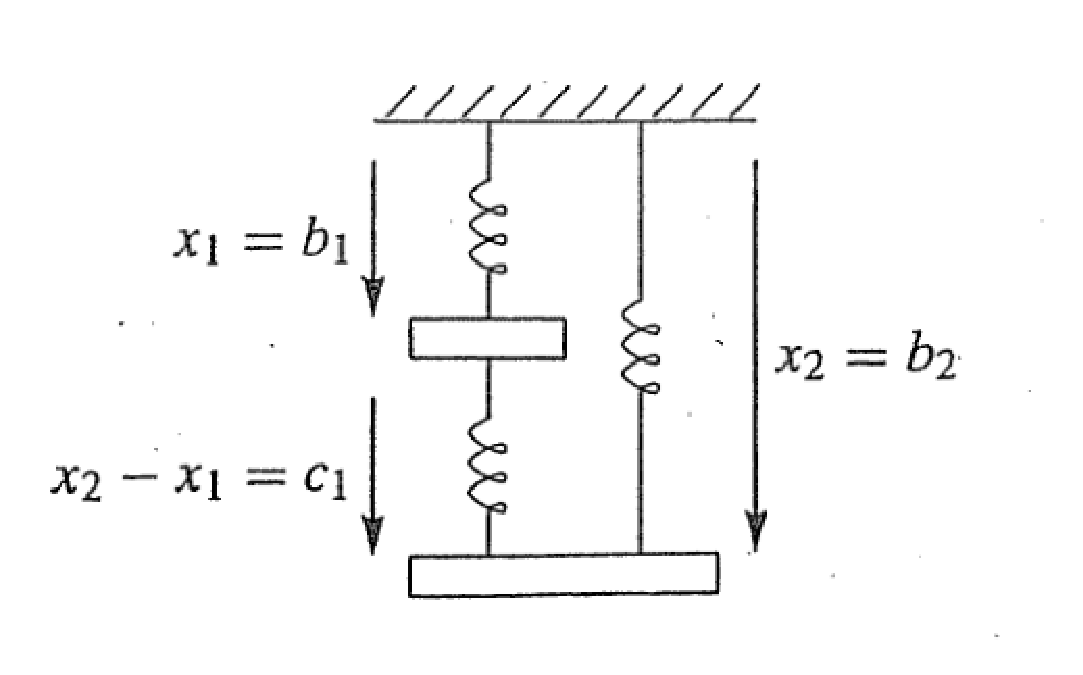
\includegraphics[width=0.7\linewidth]{TeX_files/Part02/chapter04/image/4-4}
		\caption{观测方程和状态方程的质量弹簧当量}
		\label{fig:4-4}
	\end{figure}	
	卡尔曼在每个预测/校正中增加一个弹簧 
	\begin{equation*}
	\hat{x}_{1|1}=b_1  \qquad  \hat{x}_{2|1}=b_1+c_1
	\end{equation*}
	\begin{equation*}
	\hat{x}_2=\hat{x}_{2|2}=\frac{1}{3}(b_1+2b_2+c_1)
	\end{equation*}
	
	解法 \quad  (4.30)中加权最小二乘原则仍给出$\hat{x}_1$和$\hat{x}_2$,最小化为:
	\begin{equation}
	E=\frac{1}{\sigma^2_1}(b_1-x_1)^2+\frac{1}{v^2_1}(c_1+x_1-x_2)^2+\frac{1}{\sigma^2_2}(b_2-x_2)^2
	\end{equation}
	
	加权正常方程$A^TCA=A^TCb$将有$C^{-1}=diag(\sigma^2_1,v^2_1,\sigma^2_2)$,有$C=I,\sigma_1=\sigma_2=V_1=1$:
	\begin{equation}
	\begin{bmatrix}
	\hat{x}_1  \\ \hat{x}_2
	\end{bmatrix}
	=
	\begin{bmatrix}
	b_1-c_1  \\  b_2+c_1
	\end{bmatrix}
	\end{equation}
	给出:
	\begin{equation*}
	\hat{x}_1=\frac{1}{3}(2b_1+b_2-c_1)
	\end{equation*}
	\begin{equation*}
	\hat{x}_2=\frac{1}{3}(b_1+2b_2+c_1)
	\end{equation*}
	
	最新的估计$\hat{x}_2$给了最新的观测值$b_2$一个较大的权重$\frac{2}{3}$。
	
	现在递归计算。关键的一点是$A^TCA$是三对角矩阵(在第8章中,当状态x是一个向量时,它将成为块对角矩阵)。观测方程$A_ix_i=b_i$与状态方程$x_{i+1}=F_ix_i+c_i$相连接,在三对角矩阵$A^TCA$中前向消去法总是一个递归乘法器和一个支点,然后回代是第二个递归,落后于时间。
	
	关键是事实本身,前向递归在观测方程、多达状态方程、还包括时间t=i的基础上,找到最佳估计$\hat{x}_{i|i}$,通常情况下,最终状态的估计$\hat{x}_{n|n}$是我们想要的,然后忘记回代这一步。
	
	回代这一步是调整先前的$\hat{x}_{i|i}$去解释之后的观测方程和状态方程,在时间i之后,以这种方式返回被称为“平滑”,它会使正常方程$A^TCA\hat{x}=A^TCb$产生正确的答案$\hat{x}_{i|n}$。
	
	甚至说寻找$\hat{x}_{i|i}$的前向递归是一个两步法。先前的一步$\hat{x}_{i-1|i-1}$通过时间$i-1$使用所有的信息,接下来状态方程给出一个预测,然后观测值$b_i$加上一个校正,与卡尔曼的滤波一起产生$\hat{x}_{i|i}$,预测和校正为:
	\begin{equation*}
	\hat{x}_{i|i-1}=F_{i-1}\hat{x}_{i-1|i-1}+c_i
	\end{equation*}
	\begin{equation*}
	\hat{x}_{i|i}=\hat{x}_{i|i-1}+K_i(b_i-A_i\hat{x}_{i|i-1})
	\end{equation*}
	该校正像使用增益矩阵$K_i$更新一样被写入,新数据是$c_i$和$b_i$,我们通过最小二乘,一次增加一个方程求解这个完整的系统$Ax=b$。
	
	在递归最小二乘中,有更多的一些东西需要我们计算——估计$\hat{x}_{i|i}$的可信度。协方差矩阵$P_{i|i}=(A^TCA)^{-1}_i$也是递归更新,卡尔曼滤波的每一步都增加一行(或块)到A和C中,一列(或块)到$A^T$和$C$中。预测校正步骤计算$P_{i|i-1}$和$P_{i|i}$,在$\hat{x}_{i|i-1}$和$\hat{x}_{i|i}$中的误差协方差。
	
	公平地说,卡尔曼滤波变得复杂,即使这个计划一直向前。所有的作者试图找到一个清晰的方法去推导$\hat{x}_{i|i}$和$P_{i|i}$的矩阵公式(有多种方式给数值以不同的递归)。平方根滤波用$LDL^T$或$QR$来减少当方差变得很小或很大时的数值不稳定性,我们对卡尔曼滤波的阐述将在第八章进行。
	
	最重要的一点是,协方差矩阵$P_{i|i}$像状态$x_i$具有相同的大小,这个大小与在第i步的观测数量$m_i$无关,如果我们更新最佳拟合直线,我们的矩阵保持2乘以2。
	
	例4.7 \quad (心率)在C=I(单位方差)下,递归找出P和$\hat{x}$:
	
	从$x_1=b_1$开始:\quad\quad  $A_{1|1}=[1]$  给出 $P_{1|1}=(A^TA)^{-1}_{1|1}=[I]$

	加上$x_2-x_1=c_1$:\quad $A_{2|1}=\begin{bmatrix} 1 & 0 \\ -1 & 1 \end{bmatrix}$
	和 $(A^TA)^{-1}_{2|1}=\begin{bmatrix} 1 & 1 \\ 1 & 2 \end{bmatrix}$ 给出  $P_{2|1}=2$
	
	包括$x_2=b_2$:\quad  $A_{2|2}=\begin{bmatrix} -1 & 0 \\ -1 & 1 \\ 0 & 1 \end{bmatrix}$
	和 $(A^TA)^{-1}_{2|2}=\frac{1}{3}\begin{bmatrix} 2 & 1 \\ 1 & 2 \end{bmatrix}$ 给出  $P_{2|2}=\frac{2}{3}$。
	
	第一次估计是$\hat{x}_{1|1}=b_1$(没有平滑!),使用状态方程进行接下来预测$\hat{x}_{2|1}=b_1+c_2$,使用最后的$A_{2|2}$得到校正$\frac{1}{3}(b_1+2b_2+c_1)$。
	
	那些方差$P_{2|1}=2$和$P_{2|2}=\frac{2}{3}$是$(A^TA)^{-1}_{2|1}$和$(A^TA)^{-1}_{2|2}$的最后一项,向量$x_i$引导块的支点$P^{-1}$。这里的2和$\frac{2}{3}$也被看作$b_1+c_1$和$\frac{1}{3}(b_1+2b_2+c_1)$的系数平方和。
	
	回代(平滑)在(4.32)中,调整$\hat{x}_{1|1}=b_1$成为$\hat{x}_1=\frac{1}{3}(2b_1+b_2-c_1)$。